

%!TEX root = ./main.tex
\chapter{Of Server Sockets and their Characteristics 
\label{chapter:sockets}}

%%%%%%%%%%%%%%%%%%%%%%%%%%%%%%%%%%%%%%%%%%%%%%%%%%%%%%%%%%%%%%%%%%%%%%%%%%%%%%%%
% SERVER SOCKETS
%%%%%%%%%%%%%%%%%%%%%%%%%%%%%%%%%%%%%%%%%%%%%%%%%%%%%%%%%%%%%%%%%%%%%%%%%%%%%%%%
\section{Server Sockets} Since the Internet has moved from a research project to a widely used, public communication infrastructure, one of the critical success factors was its diversity with respect to network applications or services. This was heavily favored by the Internets layered design as described by the \gls{osi}. 

Todays network applications ranges from traditional services as web, \gls{FTP} 
or mail to new and emerging services as video streaming and social networks. 
However, the terms \emph{network application} or \emph{network service} are 
overloaded and are used differently depending on the actual technical context.

By relying on flow-level data, information of layer 5-8 of the \gls{osi} are not available in the data set. Therefore, network services can be differentiated only by information of layer 3 and 4 of the \gls{osi}. For this reason, the following abstractions of a connection end-point are defined:
%%%%%%%%%%% SOCKET DEFINITION 			%%%%%%%%%%%%%%%%%%%%%%
\parbox{ 
\textwidth}{ 
\begin{defn}
	{\textbf{Socket}\\} A socket is uniquely defined by the triple (\textbf{IP address}, \textbf{IP protocol number} and \textbf{protocol port number}). In this context, a socket is only defined for IP protocol \gls{TCP}(6) and \gls{UDP}(17). 
\end{defn}
}
%%%%%%%%%%% SERVER SOCKET DEFINITION 	%%%%%%%%%%%%%%%%%%%%%%
\parbox{ 
\textwidth}{ 
\begin{defn}
	{\textbf{Server Socket 
	\label{def:serversocket}}\\} A server socket is a socket with a process listening to incoming connections and thus offering a network service. The lifetime of a server socket is not restricted to individual connections, but by the lifetime of the network service. 
\end{defn}
}

%%%%%%%%%%% CLIENT SOCKET DEFINITION 	%%%%%%%%%%%%%%%%%%%%%%
\parbox{ 
\textwidth}{ 
\begin{defn}
	{\textbf{Client Socket}\\} A client socket is a socket which is only used to 
	initiate and collate a connection to a server socket. Therefore, a client 
	socket is of temporary lifetime which is determined by the duration of the 
	connection t the server socket. 
\end{defn}
}

In spite of the containment of the term \emph{server}, definition 
\ref{def:serversocket} is not only valid for classical server-client 
applications as \gls{HTTP}, \gls{FTP}, or \gls{SSH}, but also holds for 
\gls{p2p} applications. Furthermore, the definition allows completely symmetric 
server-server connections as for example \gls{NTP} as well. 


%%%%%%%%%%%%%%%%%%%%%%%%%%%%%%%%%%%%%%%%%%%%%%%%%%%%%%%%%%%%%%%%%%%%%%%%%%%%%%%%
% DETECTION OF SERVER SOCKETS
%%%%%%%%%%%%%%%%%%%%%%%%%%%%%%%%%%%%%%%%%%%%%%%%%%%%%%%%%%%%%%%%%%%%%%%%%%%%%%%%
\section{Detection of Server Sockets 
\label{section:socket_detection}}

% problem of detection with flow-level information (timing issue + flags)
Basically, a \gls{server socket} can be identified by the fact that a client 
opens a socket which initiates a connection to a \gls{server socket}. Usually, 
a \emph{client socket} is chosen at random by his operating system and the 
\gls{server socket} is statically allocated over the lifetime of network 
service process. Moreover, on each host a socket can only be assigned to one 
specific process per instance, i.e. a client socket connection initializing 
application or a \glspl{server socket} network application waiting on client 
connections. Otherwise, a socket-in-use-error is issued by the operating 
system\citep{Schatzmann:Dissection}.

A straight-forward approach for detecting \glspl{server socket} is to infer the 
initiator of the connection by the timing information and determine its opposite 
as the \gls{server socket}. However, this approach requires a time 
synchronization of all flow exporting devices across the network. In practice, 
this can be hardly achieved in a satisfactory and reliable way so that all 
timing errors are corrected as shown by \citet{Trammell}.

% connection graph idea... +image
Besides the classification method based on well known ports  
\citet{Schatzmann:Mining,Schatzmann:Dissection,Schatzmann:Tracing} proposed a 
heuristic, greedy approach for detecting \glspl{server socket} with flow-level 
data. The central idea of this approach is to build a bipartite communication 
graph, assume that server sockets act as concentrator, and then to greedy solve 
a minimum vertex cover problem for extracting concentrators. 

A bipartite connection graph as shown by figure \ref{fig:bipartite_graph} 
consists of nodes each representing an unique socket. If a bidirectional 
connection between two sockets is observed, an undirected, unweighted edge 
between the corresponding two nodes is assigned. This means that neither the 
direction nor the weight in terms of packets or bytes are required at all to 
build the connection graph. 

\begin{figure}
	[h] \centering 
	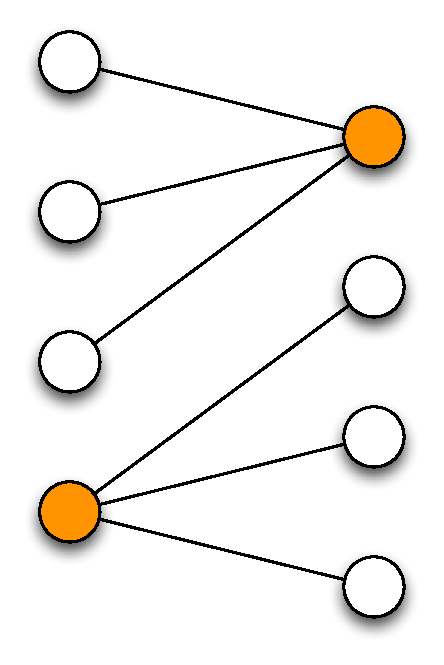
\includegraphics[width=\linewidth/3]{images/connection_graph.eps} \caption{Example of a bipartite connection graph with two concentrators of degree 3 marked as orange} 
	\label{fig:bipartite_graph} 
\end{figure}

In consequence of the fact that \glspl{server socket} provide a network 
application or service, they are likely to be contacted by several clients 
depending on their popularity. To this end, a socket which is contacted by a 
certain amount of client sockets and thus have a high degree in the connection 
graph is defined to be a \textbf{concentrator}. These concentrators are likely 
to offer a network service and are thus \glspl{server socket}. 
This approach is able to detect \glspl{server socket} which are offering not 
only classical client-server services running on well known ports, such as web, 
\gls{FTP}, or \gls{SSH}, but also \gls{p2p} applications such as for example 
Skype and Bit-torrent super-nodes.

% introduce minimal vertex cover problem
\todo{Describe algorithm}

% greedy algorithm to solve mvcp
% recalling sockets for optimization
\begin{algorithm}[t!]
\caption{Detection of server sockets by \citet{Schatzmann:Mining,Schatzmann:Dissection, Schatzmann:Tracing}}
\label{alg:service_tracing_ss-detection}
\begin{algorithmic}
\STATE
\STATE compute list $SS_{in}$ \COMMENT{int. sockets sorted by \# ext. clients}
\STATE compute list $SS_{out}$ \COMMENT{ext. sockets sorted by \# int. clients}
\STATE
\WHILE{(deg($SS_{out}[0]$) $ > 2 $ \OR deg($SS_{in}[0]$)$ > 2$)}
    \WHILE {(deg($SS_{in}[0]$) $ > $ deg($SS_{out}[0]$))}
        \STATE $ss$ = $SS_{in}[0]$ \COMMENT{classify $ss$ as internal server socket}
        \STATE remove $ss$ from $SS_{in}$
        \STATE update deg() for all entries of $SS_{in}$
    \ENDWHILE
    \WHILE{(deg($SS_{out}[0]$) $ \geq $ deg($SS_{in}[0]$))}
        \STATE $ss$ = $SS_{out}[0]$ \COMMENT{classify $ss$ as external server socket}
        \STATE remove $ss$ from $SS_{out}$
        \STATE update deg() for all entries of $SS_{out}$
    \ENDWHILE
\ENDWHILE
\end{algorithmic}
\end{algorithm}

\begin{figure}
	[ht] \centering
	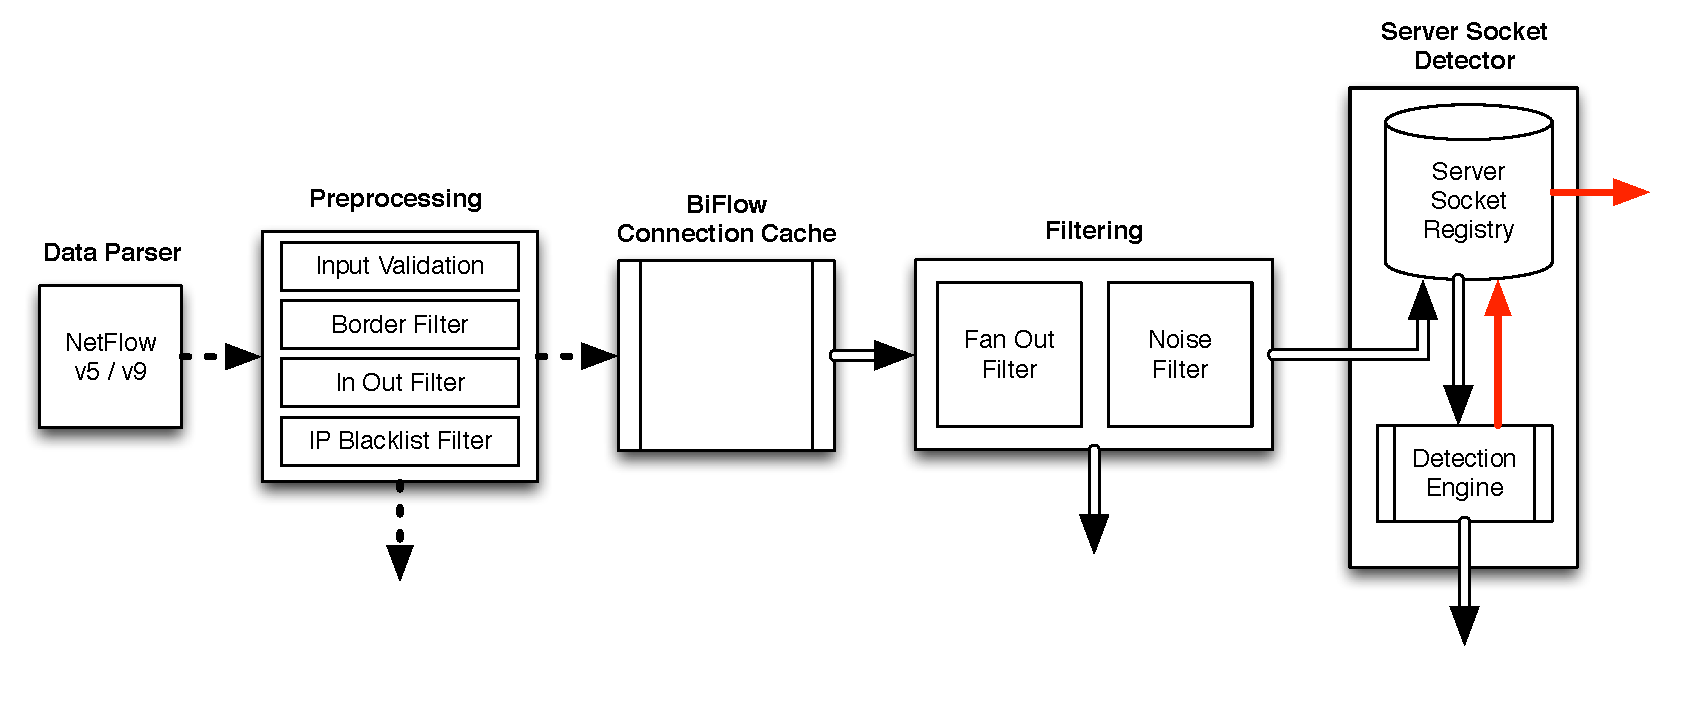
\includegraphics[width=\linewidth]{images/Detection_chain.eps}
	\caption{Processing chain for server socket detection} 
	\label{fig:detection_chain} 
\end{figure}

\subsection{Implementation}
Figure \ref{fig:detection_chain} illustrates the processing steps of the 
overall detection chain. The data parser is responsible to read the netflow data 
either in NetFlow v5 or NetFlow v9 format. These unidirectional flow records are 
then preprocessed by different blocks. While the input validator is performing 
some basic sanity checks of the flow data, the preprocessing filters are 
limiting the number of flows to the required kind of flow data. On the one hand, 
the border filter is removing all flow records not generated by a border router 
interface to efficiently prevent duplicate flow records. On the other hand, the 
In-Out filter is removing all non cross-border traffic, i.e. transit traffic 
(external to external) or entirely internal traffic (internal to internal). 
Furthermore, the IP blacklist filter is removing traffic towards blacklisted IP 
addresses or networks.

The connection cache is responsible for summarizing all related unidirectional 
flow records into a single bidirectional flow record during a certain caching 
interval. After this caching step, these bidirectional flows are filtered by a 
fan-out filter implementing the idea of \citet{Allman:2007} to mitigate the 
effects of scanning and \gls{p2p} churn. This scanning filter is discussed in 
more detail by \citet{Schatzmann:Mining,Schatzmann:Dissection, 
Schatzmann:Tracing}. 

Afterwards, the remaining bidirectional flow records are again reduced by the 
noise filter. This last filtering module is responsible to filter bidirectional 
flow records which does not represent a correct bidirectional connection. A 
correct bidirectional connection is simply defined as either a correct \gls{TCP} 
handshake or a reply flow as in case of \gls{UDP}. 
Hence, the approach of deducing correct connections is to investigate the number 
of packets for each direction of the bidirectional flow record, i.e. the 
outgoing and the incoming flow record, since there are only cross-border flows 
remaining due to the In-Out filter. 
If a bidirectional \gls{TCP} flow has in a single direction less than 3 
packets, the filter assumes that this flow does not represent a correct 
connection and is filtering this record. Accordingly, a bidirectional \gls{UDP} 
flow is required to consist of at least 1 packet for each direction.

After these filtering steps, the remaining bidirectional flows are passed to the 
\emph{server socket detector} which is finally performing the 
\gls{server socket} detection approach previously discussed. Generally, the 
\emph{server socket detector} is build from two main parts. 
On the one side, there is the \emph{server socket registry} which is 
containing all already known \glspl{server socket}. On the other side, the 
detection engine implements the \gls{server socket} detection algorithm. 

Firstly, the sockets of all bidirectional flows are queried against the current 
\emph{server socket registry} for checking if they are already known. If this is 
the case, the corresponding bidirectional flow records are removed and only the 
remaining flow records are passed to the detection engine to increase the 
efficiency of the detection algorithm. 
The detection engine builds the bipartite connection 
graph and is detecting the concentrators of it. These detected \glspl{server 
socket} are then passed to the \emph{server socket registry} so that these 
sockets may be recalled afterwards. 

Finally, the \emph{server socket registry} is able to output all detected 
\glspl{server socket} of the observation period. 

%%%%%%%%%%%%%%%%%%%%%%%%%%%%%%%%%%%%%%%%%%%%%%%%%%%%%%%%%%%%%%%%%%%%%%%%%%%%%%%%
% MONITORING OF SERVER SOCKETS
%%%%%%%%%%%%%%%%%%%%%%%%%%%%%%%%%%%%%%%%%%%%%%%%%%%%%%%%%%%%%%%%%%%%%%%%%%%%%%%%
\newpage
\section{Monitoring of Server Sockets 
\label{section:socket_tracking}}

The previous section outlined the approach of detecting \glspl{server socket}. 
This section covers the approach of monitoring flow data and generating 
statistical information such that some characteristics and properties of the 
found \glspl{server socket} can be assessed as further outlined in section 
\ref{section:characterization}.

\subsection{Server Socket Statistics}

The monitoring of the external 
\glspl{server socket} is done with help of the \emph{server socket registry} 
which is already used in the detection approach. This registry recalls all 
\glspl{server socket} which are known yet. 

Hence, all flows originated from a \gls{server socket} or flows which are 
destined for a \glspl{server socket} are monitored for compiling the socket 
statistics later used for the characterization.

In contrast to the detection approach, there are no scanning or other noise 
filters in the processing chain, because of the fact that they will remove at 
least some flows, mainly unidirectional flows, which are actually relevant for 
the statistics. 

Since the processing is based on data containing flows which are active within a 
certain time slot, the statistics are accounted on a the same discrete time 
scale, i.e. 10 minutes. 

At first, each flow is checked if it is a flow of a \gls{server socket}. If 
this is the case, the individual flow statistics are accounted to the 
corresponding specific \gls{server socket} \textbf{statistics record}. This 
includes the following entries: 

\vbox{
\begin{itemize}
	\item number of bidirectional connections 
	\item number of outgoing unidirectional connections 
	\item number of incoming unidirectional connections 
\end{itemize}
}

In second step, the statistics records of each discrete time slot are aggregated 
in such a way that the information of the activity within a certain time slot is 
kept. Thus, the overall \gls{server socket} statistics record contains the 
following entries: 

\vbox{
\begin{itemize}
	\item sum of bidirectional connections of each time slot 
	\item sum of outgoing unidirectional connections of each time slot 
	\item sum of incoming unidirectional connections of each time slot 
	\item number of days with connections 
	\item number of discrete time slots with connections 
	\item timestamps of discrete time slots with connections 
\end{itemize}
}

\subsection{Traffic Statistics} 

Besides of the individual \gls{server socket} statistics report, overall traffic 
statistics are accounted, mainly for deducing knowledge of how good the 
monitoring capability of the \glspl{server socket} in the \emph{server socket 
registry} is. For this reason, each flow which belongs to a \gls{server socket} 
which is present in the \emph{server socket registry} is denoted as monitored. 
Hence, flows which do not belong to a \gls{server socket} are accounted as not 
monitored. 

Moreover, all unmonitored flows can be further investigated for a better 
understanding of the type of this unmonitored traffic. This can be done on the 
following three scopes: 
\begin{itemize}
	\item protocol level 
	\item port level for \gls{UDP} and \gls{TCP} flows 
	\item location of the connection end-points 
\end{itemize}

The first scope captures statistical information of the problem that 
\glspl{server socket} are only defined for protocol \gls{TCP} and \gls{UDP}, 
hence all flows with another protocol are per definition unmonitored.

Secondly, there are statistics generated for all unmonitored \gls{TCP} or 
\gls{UDP} flows which do not have a corresponding \gls{server socket} in the 
\emph{server socket registry} present. There are various reasons for this, 
mainly related to the detection approach outlined in section 
\ref{section:socket_detection}. In most of the cases, the sockets are not 
contacted by enough clients, therefore, the are not detected as concentrators 
and in consequence of that not denoted as \glspl{server socket}. Furthermore, 
scanning activity is also a major contributor to this unmonitored flows, since 
scanning traffic and other non-legitimate traffic is removed before the 
\gls{server socket} detection is performed. Consequently, these scanned sockets 
are not detected as \glspl{server socket}, in case there is no legitimate 
traffic towards these sockets. Nevertheless, this scanning traffic is considered 
in this monitoring phase as well. 

On the one hand, there is the possibility to account for each port the 
unmonitored flows which will lead to very detailed statistical information about  
missed \glspl{server socket}. However, this comes at the price of an inefficient 
processing and higher memory usage. 

On the other hand, the flows can be categorized by port ranges. In the thesis at 
hand, there are just two ranges defined for this categorization:

\begin{itemize}
	\item low port: 0-1023 
	\item high port: 1024-65365 
\end{itemize}

These categories are further divided by the location of the socket either 
internal or external and thus involving the third scope. Hence, the unmonitored 
\gls{TCP} and \gls{UDP} flows by the following four categories:

\vbox{
\begin{itemize}
	\item external port high, internal port high 
	\item external port high, internal port low 
	\item external port low, internal port high 
	\item external port low, internal port low 
\end{itemize}
}

All these general traffic statistics allows to deduce insights about the 
properties of the detection process by learning what is missed. Moreover, these 
general traffic statistics are revealing information about the properties of the 
current \gls{server socket} set with respect to traffic representation and thus 
about some properties of this set. 

\subsection{Implementation}

Figure \ref{fig:monitoring_chain} shows the modular implementation of the 
\gls{server socket} monitoring chain. Comparing the monitoring chain to the 
detection chain from figure \ref{fig:detection_chain} it is clearly visible that 
the modules up to the bidirectional connection cache are shared. However, in the 
monitoring chain there are no fan-out filter and noise filter applied. This is 
because every traffic destined to a \gls{server socket} should be considered, 
therefore no flow records are filtered before accounting them. The 
\emph{server socket monitor} is accounting the general traffic statistics as 
well as the individual \gls{server socket} statistics.

First of all, the bidirectional flow records are separated into those belonging 
to a known \gls{server socket}, denoted as monitored traffic, and those not 
belonging to known \gls{server socket}, denoted as unmonitored traffic. 
To be more precisely, this is done by querying the \emph{server socket registry} 
which is loaded with previously detected \glspl{server socket}. Then, the 
traffic monitor investigates the monitored and unmonitored traffic for 
generating the overall traffic statistics. 
Furthermore, it examines the unmonitored traffic even more closely for deducing 
knowledge about the other traffic statistic scopes as protocol, direction 
ports and location.

\begin{figure}[hb]
	\centering
	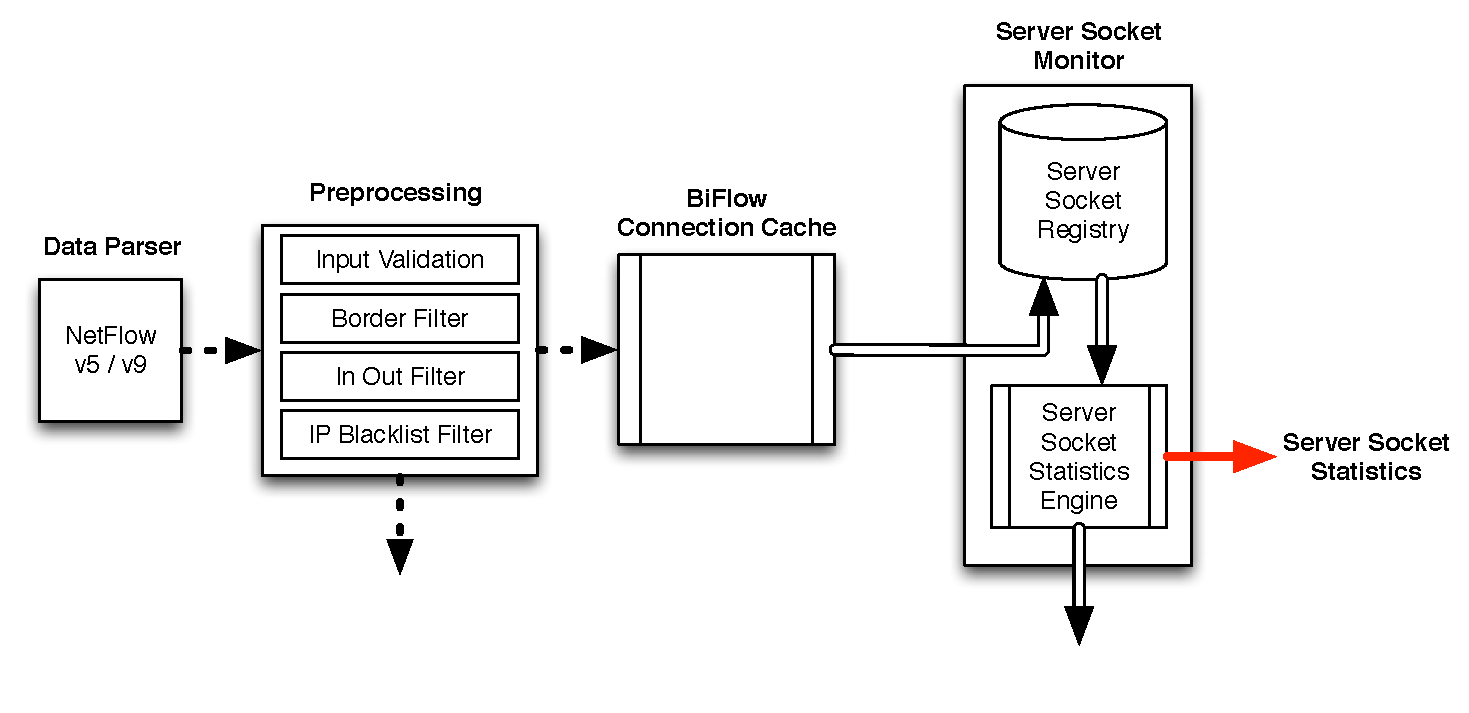
\includegraphics[width=\linewidth]{images/TrackingChain.eps}
	\caption{Processing chain for the server socket monitoring} 
	\label{fig:monitoring_chain} 
\end{figure}

%%%%%%%%%%%%%%%%%%%%%%%%%%%%%%%%%%%%%%%%%%%%%%%%%%%%%%%%%%%%%%%%%%%%%%%%%%%%%%%%
% CHARACTERIZATION SERVERSOCKETS
%%%%%%%%%%%%%%%%%%%%%%%%%%%%%%%%%%%%%%%%%%%%%%%%%%%%%%%%%%%%%%%%%%%%%%%%%%%%%%%%
\newpage
\section{Characterization of Server Sockets 
\label{section:characterization}} The main interest of this thesis is to characterize \glspl{server socket} by its \textbf{stability}, its \textbf{visibility} and its \textbf{popularity}. These properties try to address the following characteristics of a \gls{server socket}:

\vbox{ 
\begin{itemize}
	\item \textbf{Stability:} How stable is the \gls{server socket} regarding its responsiveness or availability?
	\item \textbf{Visibility:} How frequently is the \gls{server socket} contacted by other socket?
	\item \textbf{Popularity:} How many distinct sockets are contacting the \gls{server socket}?
\end{itemize}
}

These three characteristics are directly deducible from the statistics observed 
by the passive monitoring technique outlined in \ref{section:socket_tracking}. 
In the following, the three characteristics are briefly discussed.

\subsection{Stability of a Server Socket} Because of the definition and its 
detection approach a \gls{server socket} is offering a bidirectional service 
which means that the client and the \gls{server socket} are both sending 
packets. Usually, a client socket is opening the connection to a \gls{server 
socket} which will reply in return to this request. Generally, this also holds 
for \gls{p2p} applications as for example bit torrent. Therefore, a 
\gls{server socket} -- or the communication of it -- can be characterized as 
stable if it responds to all connection attempts. If a connection attempt to a \gls{server socket} is responded by the \gls{server socket}, the bidirectional connection is denoted as \textbf{balanced}. 

%%%%%%%%%%% Balanced Connection DEFINITION 	%%%%%%%%%%%%%%%%%%%%%%
\parbox{ 
\textwidth}{ 
\begin{defn}
	{\textbf{Balanced Connection}\\} A connection between two sockets is balanced, if there is one flow originating from each socket which is destined for the other socket. Hence, the connection is bidirectional with two corresponding unidirectional flows. 
\end{defn}
}

Thus, the overall stability \gls{server socket} or availability of its service 
can be approximated by the ratio of the balanced to all connections destined to 
this \gls{server socket}, i.e. the balanced and the unbalanced. This ratio is 
referred as a \gls{server socket} \textbf{stability ratio} and is mathematically 
defined by equation \ref{eq:ratio}. 
\begin{equation}
	\text{Stability}(\text{Socket}_i) = \frac{\text{balanced connections}(\text{Socket}_i)}{\text{balanced connections}(\text{Socket}_i) + \text{unbalanced connections}_{in}(\text{Socket}_i)} 
	\label{eq:ratio} 
\end{equation}

Hence, a \gls{server socket} with a stability ratio of 1 does only have 
bidirectional connections and thus, replies to all connection attempts. On the 
other side, a stability ratio of 0 indicates that there are only connections 
attempts by client sockets, but the \gls{server socket} never replied upon these 
request. Unbalanced outgoing connections from the \glspl{server socket} are 
indicating a client error or scanning activities of clients with spoofed 
(internal) source address which are not observed by the monitoring system. 
Therefore, these unbalanced outgoing connections are not considered for 
determining the stability ratio at all.

\subsection{Visibility of a Server Socket\label{subsection:visibility}}

% discrete time slots activities of a socket, per day, per 5min slot?
% distribution is heavy-tailed, alot of sockets only rarely connected => due to scanning? due to malware?
The monitoring process of the \glspl{server socket} is done passively, thus if a 
\gls{server socket} is visible in the flow-level data of a certain time period, 
the \gls{server socket} is active during at that time. Hence, the visibility of 
a \gls{server socket} during a certain time interval $t+\Delta{t}$ is a binary 
measure, either inactive in case it is not visible or active in case it is 
visible in the data set. Equation \ref{eq:visibility} defines the visibility of 
a socket during the time interval $t+\Delta{t}$: 
\begin{equation}
	\text{Visibility}_t(\text{Socket}_i,t+\Delta{t}) = \left\{ 
	\begin{array}{l l}
		1 & \quad \text{if $\text{Socket}_i$ is active during $t+\Delta{t}$}\\
		0 & \quad \text{if $\text{Socket}_i$ is not active during $t+\Delta{t}$}\\
	\end{array}
	\right. 
	\label{eq:visibility} 
\end{equation}

In consequence, there are different granularities $\Delta{t}$ to define the 
visibility of a \gls{server socket}. On the one hand, the most fine-grained 
resolution is just the flow-level data cache interval. In most of the cases, 
this flow-level data cache interval is set to 300 seconds. This most 
fine-grained resolution is referred as the \emph{time slot} resolution, since 
the entire processing is based on such discrete data chunks, containing all 
flows active during this time period. 
On the other hand, there are several more coarse-grained resolutions of the 
visibility possible. An obvious is resolution of a day, i.e. 
$\Delta{t} = 86400$s.

Furthermore, the visibility of a \gls{server socket} can be extended from a 
single time period to the overall observation time, i.e. a week long trace, by 
summing up the individual visibilities of each time slot as shown in equation 
\ref{eq:visibility_sum}.
\begin{equation}
	\text{Visibility}(\text{Socket}_i) = \sum_{t} \text{Visibility}_t(\text{Socket}_i,t+\Delta{t})
	\label{eq:visibility_sum} 
\end{equation}

However, this summing approach exacerbate the comparison between different 
observations since it represents the visibility in absolute terms. Therefore, an 
even better metric for the visibility of a \gls{server socket} is to average the 
individual $\text{Visibility}_t(\text{Socket}_i,t+\Delta{t})$ as outlined by 
equation \ref{eq:visibility_avg}. This normalizes the visibility to a value in 
the range between 0 and 1, representing the ratio of its visibility to the 
maximum visibility possible. Thus, a value of 1 means that the socket is visible 
in every single time slot and a value of 0 that the socket was never active. 

\begin{equation}
	\overline{\text{Visibility}}(\text{Socket}_i) = \frac{\sum_{t} \text{Visibility}_t(\text{Socket}_i,t+\Delta{t})}{\sum_{t}1}
	\label{eq:visibility_avg} 
\end{equation}

\subsection{Popularity of a Server Socket}

% number of flows / clients?.. degree of Server Socket
Besides the visibility of a \gls{server socket}, its popularity is another major 
key characteristics. Whereas the visibility of a \gls{server socket} defines how 
frequent a socket is contacted by at least one connection endpoint, the 
popularity of a \gls{server socket} is defined by the number of connection 
attempts of client sockets during a certain period of time. The popularity of 
\gls{server socket} can be deduced by various metrics as the number of flows, 
bytes or clients.


%%%%%%%%%%%%%%%%%%%%%%%%%%%%%%%%%%%%%%%%%%%%%%%%%%%%%%%%%%%%%%%%%%%%%%%%%%%%%%%%
% ANALYSIS of SERVER SOCKETS IN THE WILD
%%%%%%%%%%%%%%%%%%%%%%%%%%%%%%%%%%%%%%%%%%%%%%%%%%%%%%%%%%%%%%%%%%%%%%%%%%%%%%%%\newpage
\section{Analysis of Server Sockets in the Wild}

This section covers an analysis of \gls{server socket} found during a 
week long data trace from 2010/11/01 00:00:00 UTC until 2010/11/06 00:49:00 UTC, 
thus covering mainly the first 5 working days in November 2010.

\subsection{Detected Server Sockets}

% sum up of detection parameters > 2 biflows per 5min interval with more TCP 
% packets > 3 UDP > 1
For detecting the \glspl{server socket} in this observation period, the 
previously discussed detection approach was applied as illustrated by figure 
\ref{fig:detection_chain}. In detail, the connection cache was configured to 
summarize all related unidirectional flow records into a single bidirectional 
flow record during an aggregation interval of 600s. 

After this caching step, these bidirectional flows are filtered by a fan-out 
filter implementing the idea of \citet{Allman:2007} to mitigate the effects of 
scanning and \gls{p2p} churn. This fan-out filter is configured to require at 
least 4 unidirectional connections with a certain host as source and at least 2 
times more unidirectional connections than bidirectional connections for 
classifying this host as a scanning host. 
Previous work\citep{Schatzmann:Mining,Schatzmann:Dissection, Schatzmann:Tracing} 
has shown that these parameters are a good choice for efficiently mitigating the 
scanning noise so that the scanning spikes of the total traffic volume are 
successfully reduced.

Moreover, the noise filter is configured to filter all \gls{TCP} flows with less 
than 3 packets in a single direction and \gls{UDP} flows with less than 1 packet 
in a single direction. 

Furthermore, the \emph{server socket detector} is configured to extract sockets 
with a degree of 2 or higher as concentrators, thus requiring two independent 
connections to a \gls{server socket} within 600 seconds. 

% state overall number of detected external and internal server sockets during 
% this period
During the entire observation period of 120.8 hours, the 
\emph{server socket detector} managed to detect 1'862'389 external 
\glspl{server socket} and 609'670 internal \glspl{server socket}.

\subsection{Gravitational Forces of Server Sockets}
% traffic statistics of server sockets detected by type and ratio of traffic 
% towards server sockets
In the following, the overall traffic statistics of the detected 
\glspl{server socket} are briefly discussed. Figure \ref{fig:flows_by_type} 
shows the absolute number of flows during the entire observation period 
separated by the type of connection. If the flow is destined to a 
\gls{server socket}, the flow is denoted as monitored, otherwise as unmonitored. 
Furthermore, the type of connection also considers the balance or direction of 
the connection, i.e. if the flow is bidirectional, unidirectional outgoing or 
unidirectional incoming. Hence, in total there are 6 possible combinations for 
the type of connection, allowing a good interpretation of the detection 
approach. For easier comparison of each type of connection, figure 
\ref{fig:monitored_flows_by_type} shows the ratio of monitored and unmonitored 
flows by the direction.

In figures \ref{fig:flows_by_type} and \ref{fig:monitored_flows_by_type}, there 
are two gaps visible around 2010/11/01 10:00 UTC and 2010/11/04 06:05 UTC. These 
gaps result from missing flow records due to router reboots, collector outages, 
and storage failures\citep{Schatzmann:Mining}.

\begin{figure}
	[ht] \centering 
	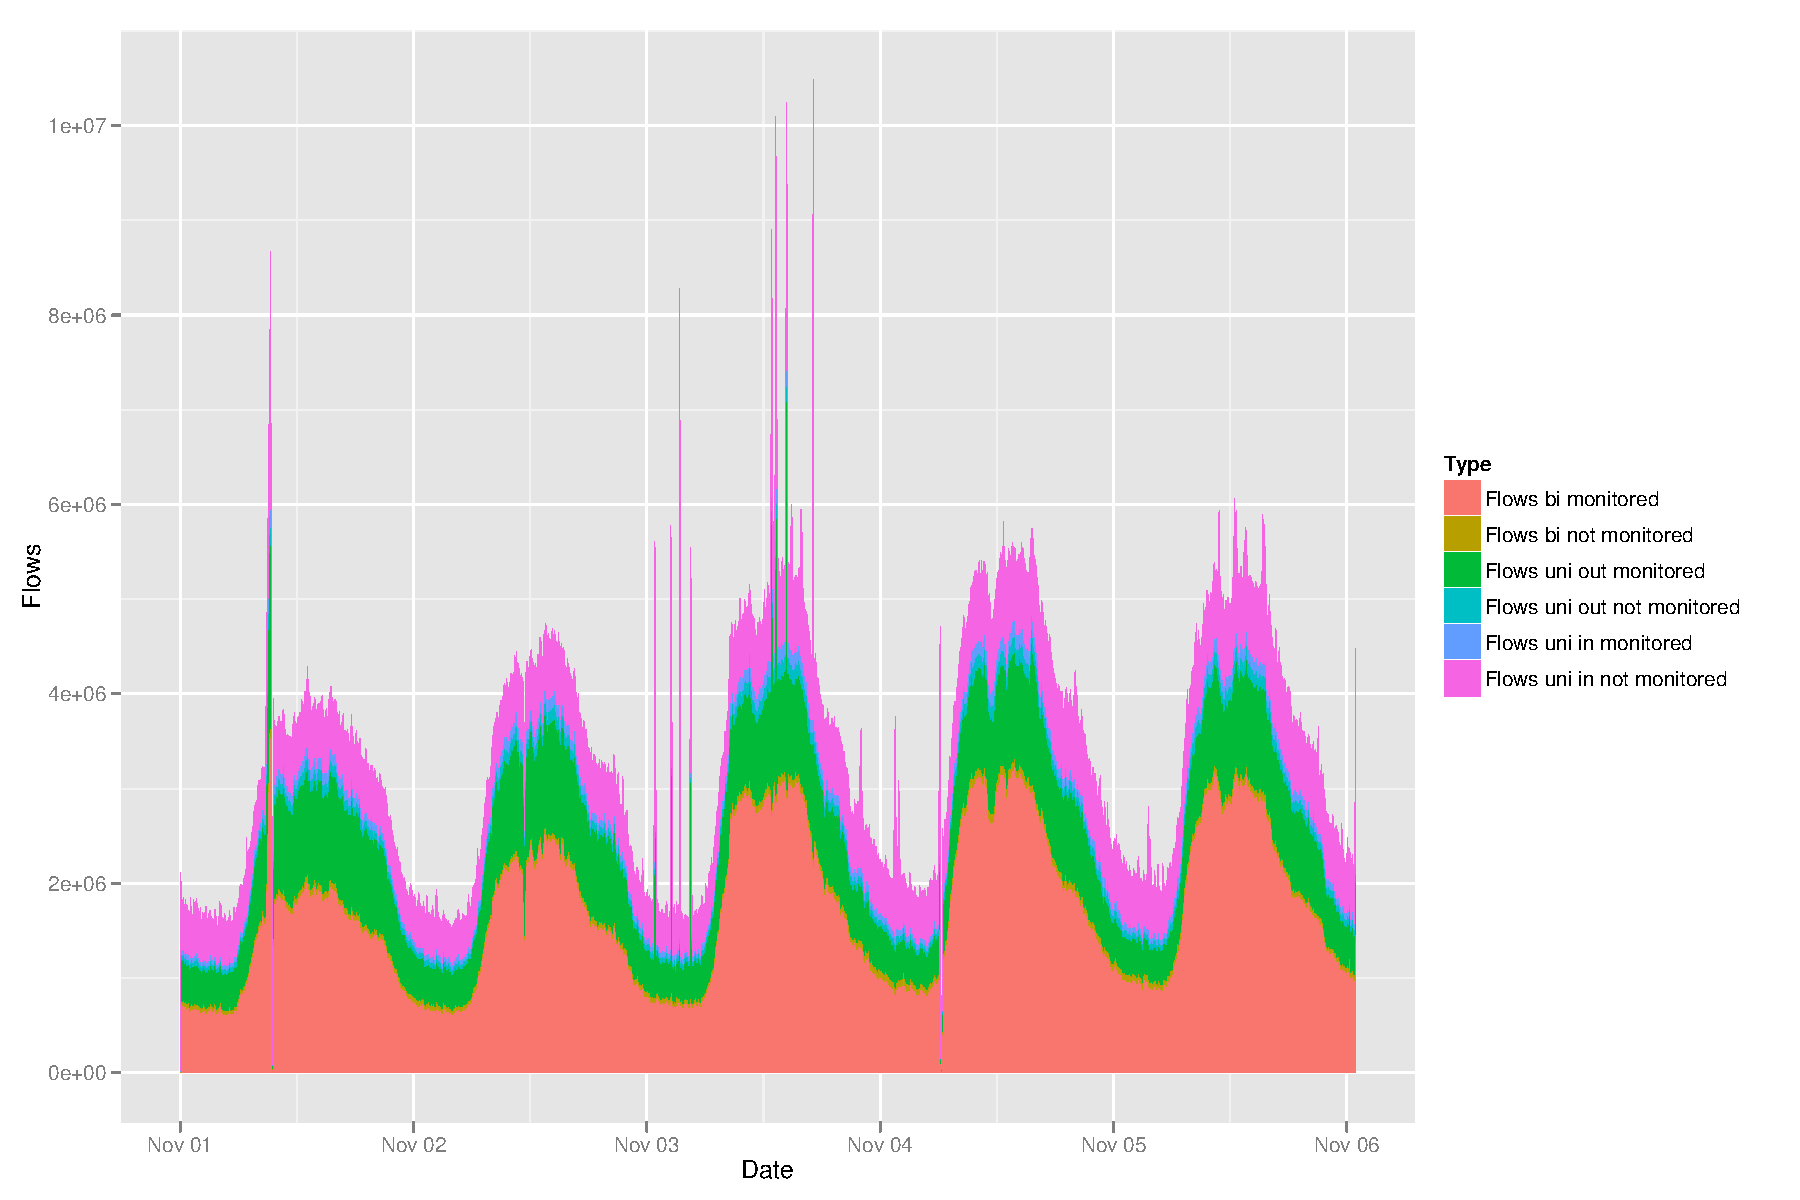
\includegraphics[width=\linewidth]{images/Flows_by_type_area_all_SeS.pdf}
	\caption{Number of flows over time by the type of connection with all detected server sockets} 
	\label{fig:flows_by_type} 
\end{figure}

\begin{figure}[h]
	\centering 
	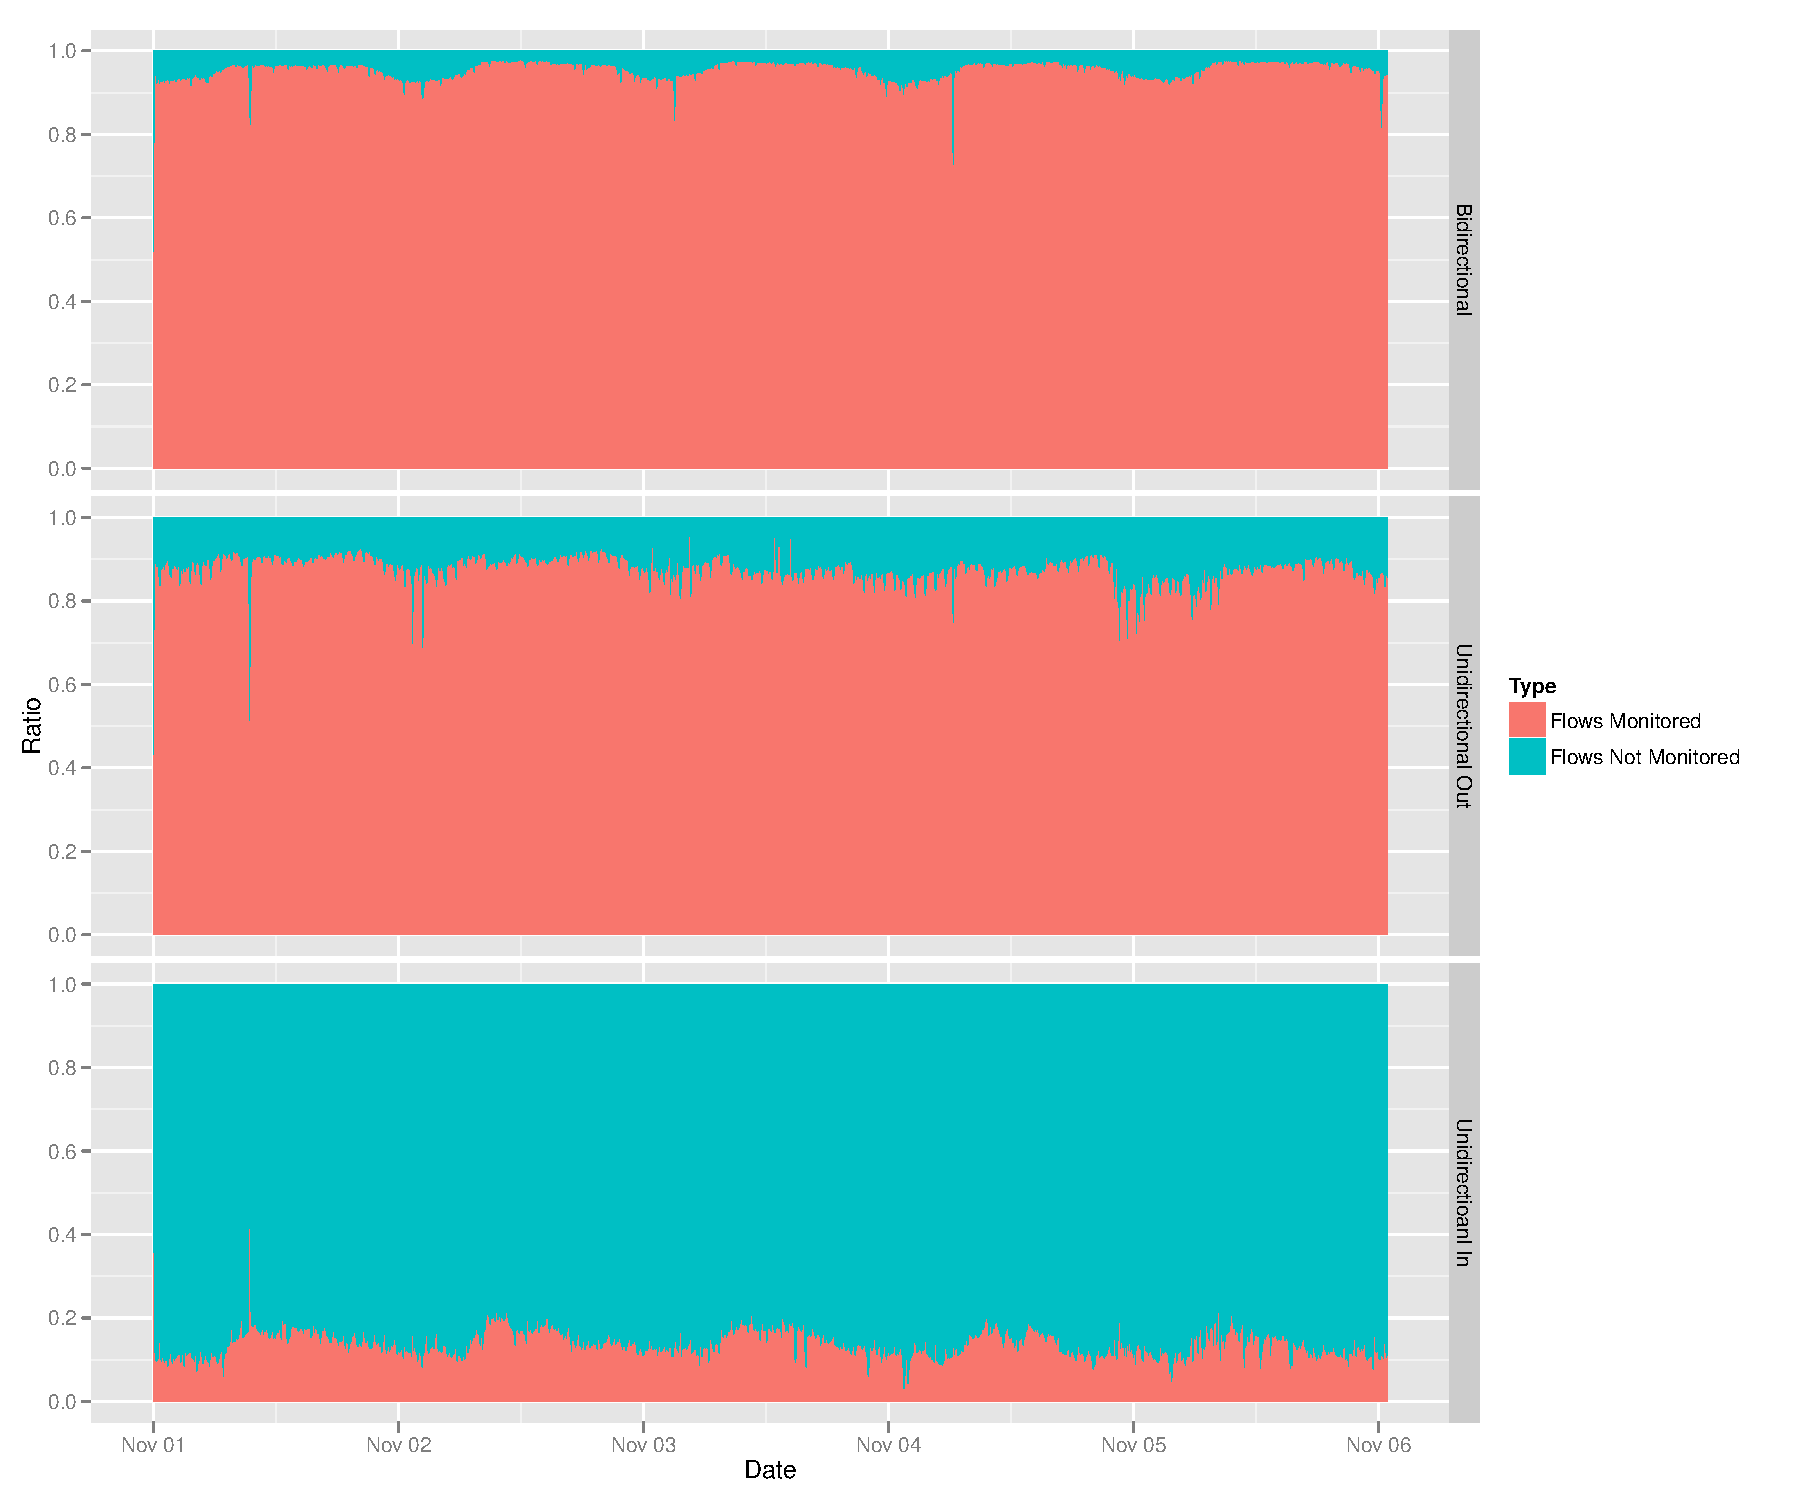
\includegraphics[width=\linewidth]{images/Flows_monitor_ratio_by_type_all_SeS.pdf}
	\caption{Flows towards known server sockets by traffic type with all detected server sockets} 
	\label{fig:monitored_flows_by_type} 
\end{figure}

Clearly, the dominating kind of the flows are the bidirectional monitored flows 
represented by the red area in figure \ref{fig:flows_by_type}. Comparing this 
share with the bidirectional unmonitored flows represented by the yellow area 
between the red and the green area, yields that the detection approach detects a 
majority of the \glspl{server socket}. This finding is even better visible on 
the bidirectional ratio of figure \ref{fig:monitored_flows_by_type}. Depending 
on the time of the day, the monitoring ratio of the bidirectional flows is 
mainly between 90\% and 97\%. 
The smaller monitoring ratios during night indicates that there is a higher 
share of unknown \glspl{server socket} active at night than during day.
A possible reason for pattern is that there are some 
\glspl{server socket} which are regularly contacted, although, only by very few 
clients so that these sockets get never more than one connection within 600 
seconds. Thus, these sockets are never detected as concentrators. 

Similarly, if the unidirectional outgoing flows are examined by looking at 
figure \ref{fig:monitored_flows_by_type}, the monitored flows have predominantly 
a high share of around 80\% to 90\% of all unidirectional outgoing flows. Figure 
\ref{fig:flows_by_type} also reveals some high peaks which are probably scanning 
or backscatter effects which are well visible at November 03 in the night and in 
the afternoon by the green spikes. However, these green peaks are categorized as 
monitored unidirectional outgoing flows. Thus, they must involve at least one 
known \gls{server socket} either located external or internal.

Finally, the unidirectional incoming flows have are predominately unmonitored 
with around 80-97\% of unmonitored flows as it can be seen in figure 
\ref{fig:monitored_flows_by_type}. The main reason for this contrast may be that 
the main part of this unidirectional incoming traffic consists of Internet 
background radiation \citep{Wustrow10,Pang04} due to malware or misconfiguration 
for example. Nevertheless, this unidirectional incoming flow traffic is 
unimportant with respect to the scope of this thesis.

In a metaphorical sense, \glspl{server socket} are comparable to masses in 
physics which are exerting gravitational forces to other objects. \Glspl{server 
socket} tend to attract a majority of the observed connections. Therefore, they 
are well suitable to represent a majority of the legitimate traffic which is 
interesting for tracking the end-to-end connectivity.

\newpage
\subsection{Characterization of Detected Server Sockets}

As discussed in section \ref{section:characterization}, this thesis proposes to 
characterize \glspl{server socket} according to their visibility, popularity and 
stability by different metrics. This section aims to deduce some statistical 
properties of the detected \glspl{server socket} regarding these 
characteristics.

\subsubsection{General Visibility of Server Sockets}

For defining a metric of the visibility of \glspl{server socket}, it is required 
to define the granularity of a observation period according to 
\ref{subsection:visibility}. For simplicity reasons, only two different 
granularities are defined. 

One the one hand, a day long observation period yields the number of visible 
days for the activity of a socket. On the other hand, an observation period of 5 
minutes is chosen, since it reflects the default processing interval of FlowBox 
and the native caching interval of the flow data. This allows a very 
fine-grained, detailed resolution of a \glspl{server socket} activity. This 
second visibility metric is referred as \emph{visible time slots(VTS)}.

\begin{figure}
	[hb] \centering 
	\includegraphics[width=\linewidth]{images/VTS_by_visibledays.pdf}
	\caption{VTS by visible days} 
	\label{fig:vts_by_visibledays} 
\end{figure}

Figure \ref{fig:vts_by_visibledays} shows the number of sockets by the visible time slots separated the number of visible days. The skewness of the 
distributions for 1 to 4 visible days are is very similar. It is obvious that 
the a socket which is visible for only one day cannot exceed 288 visible time 
slot. Nonetheless, considering this daily scaling factor, the distributions are 
looking very similar. Furthermore, figure \ref{fig:vts_by_visibledays} shows 
that the most sockets in absolute terms are only active during one day and only 
in very few visible time slots. 

However, the distribution of the number of sockets with a visibility of 5 or 
even 6 days are slightly different, since there is a higher share of sockets 
with a relatively higher visible time slots, besides the normal scaling factor 
of the number of visible days.

\subsubsection{Visibility and Stability}
Eventually, for selecting those \glspl{server socket} which are stable and often 
visible it is of importance to assess how \glspl{server socket} are distributed 
with respect to their stability and visibility characteristic. Hence, figure 
\ref{fig:rankedVisibility} shows the location of each socket in the field of the 
ranked visibility and the stability. The ranked visibility is simply defined by 
the cumulative distribution function of the visibility. Thus, a socket with a 
ranked visibility of 80\% indicates that there are 80\% of all sockets with the 
same or lower visibility than this specific socket. 

As figure \ref{fig:rankedVisibility} indicates, the sockets cluster around the 
top right corner, hence the top visible sockets tend to have a good stability as 
well.

\begin{figure}
	[hb] \centering 
	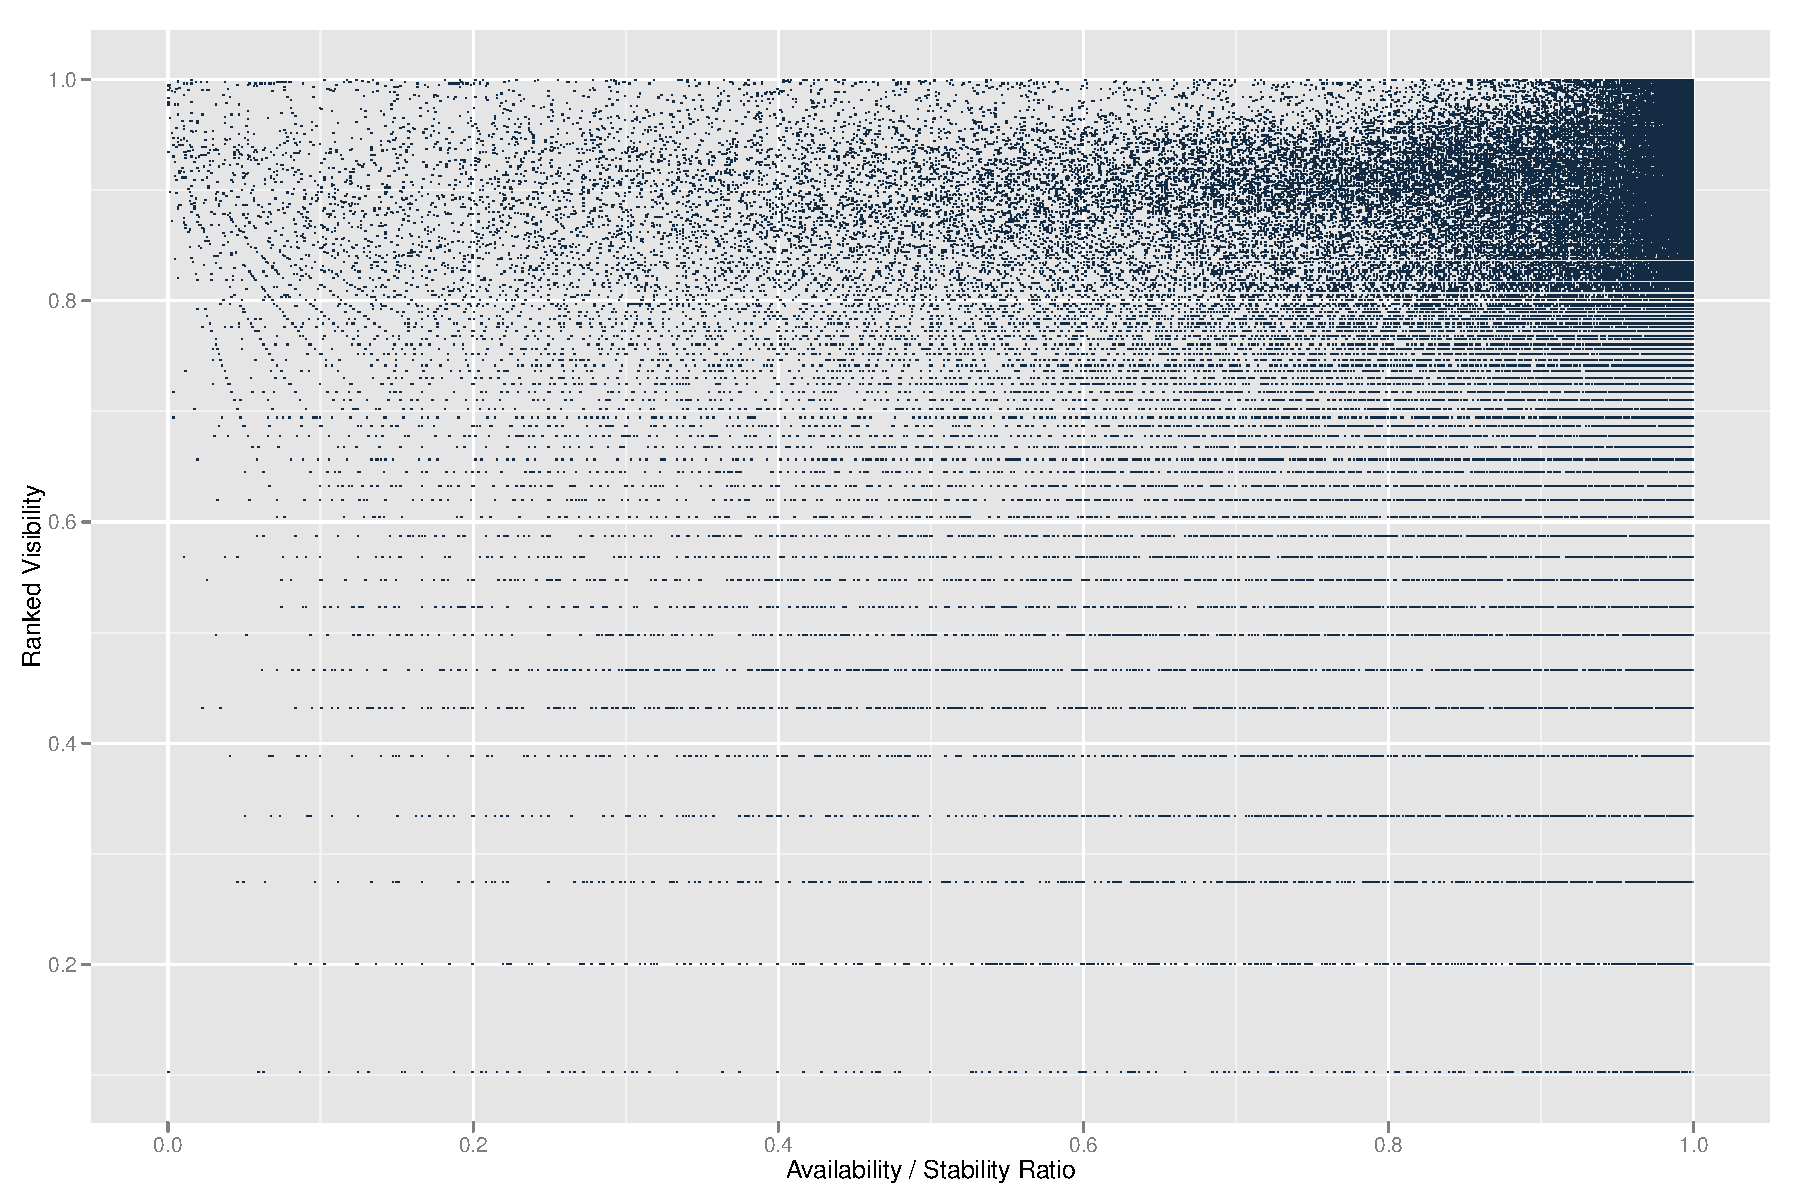
\includegraphics[width=\linewidth]{images/visibiliy_stability_map.pdf}
	\caption{Sockets by their ranked visibility and their stability} 
	\label{fig:rankedVisibility} 
\end{figure}

Furthermore, figures \ref{fig:ccdf_ratio_days} and \ref{fig:ccdf_ratio_vts} show 
each a complementary cumulated distribution function of the stability of server 
sockets with different visibilities. 

One the one side, figure \ref{fig:ccdf_ratio_days} is using the daily visibility 
of the sockets. The red curve represents the distribution of the sockets which 
are seen only in one day. Not surprisingly, these group of \glspl{server socket} 
reveal the highest share of sockets with a stability of 1. This is mainly due to 
the fact that there is a high number of \glspl{server socket} which are active 
only during a relatively short period of time. This can be justified by looking 
at figure \ref{fig:vts_by_visibledays}.

Not surprisingly there is a higher share of sockets with a visibility of 2 days 
with a stability ratio below 80\%. Intuitively, the sockets which have a good 
visibility of 5 or even 6 days tend to have a high stability as well, but they 
have a lower share of sockets which have a stability ratio of 1 than all other. 
This means that sockets which are often visible incline to have at least some 
unbalanced connections. 

On the other side, figure \ref{fig:ccdf_ratio_vts} shows the complementary 
cumulative distribution function of the stability ratio of sockets with 
different absolute visible time slots. Around 99\% of all \glspl{server socket} 
with more than 1000 visible time slots have a higher stability ratio than 95\%. 
Although, only around 20\% of them have a stability ratio of 100\%, such that 
they have no unbalanced connections at all.
As in figure \ref{fig:ccdf_ratio_days}, \glspl{server socket} with a low 
visibility incline to have a higher share of sockets with a stability ratio 
below 90\% than sockets more often visible. 

\begin{landscape}
\begin{figure}
	[p] \centering 
	\includegraphics[width=\linewidth]{images/CCDF_ratio_days.pdf}
	\caption{CCDF of the availability by visible days} 
	\label{fig:ccdf_ratio_days} 
\end{figure}
\end{landscape}

\begin{landscape}
\begin{figure}
	[p] \centering 
	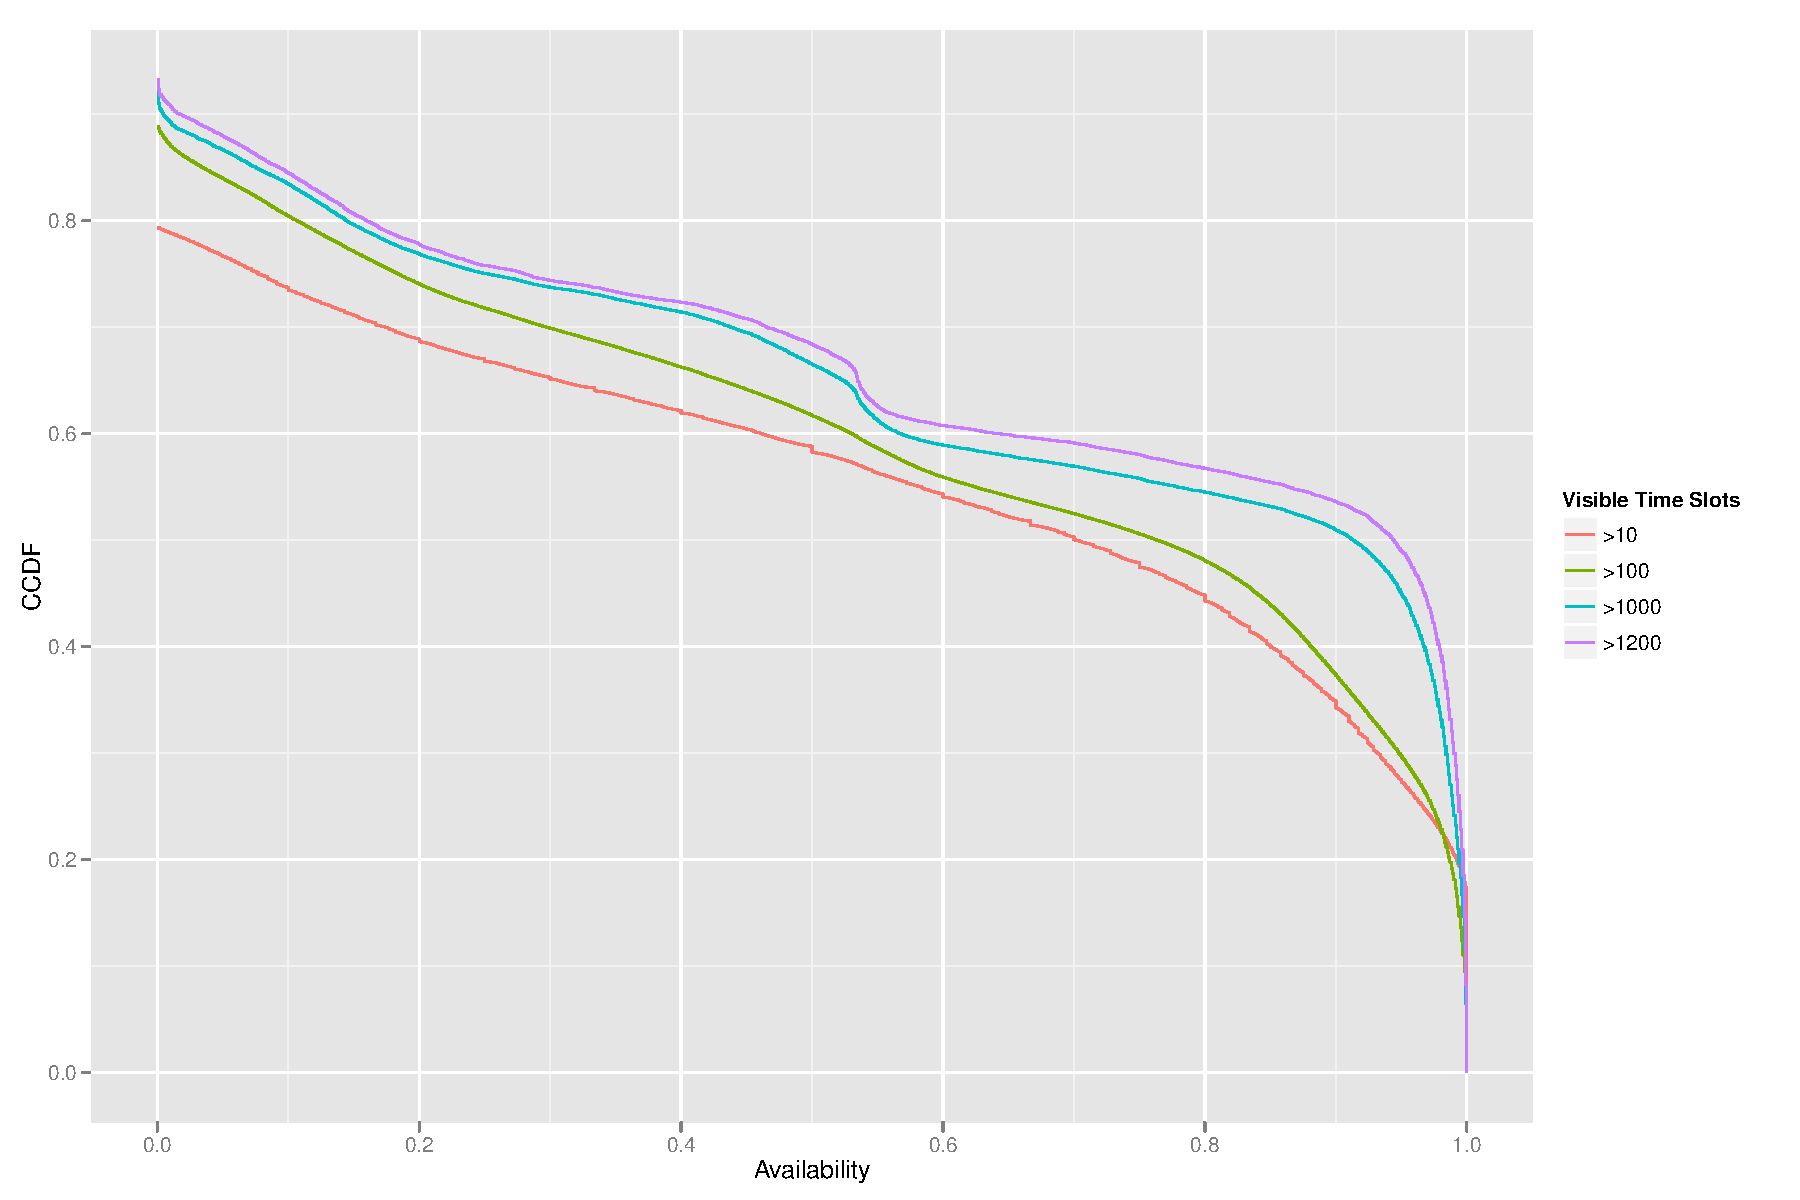
\includegraphics[width=\linewidth]{images/CCDF_ratio_VTS.pdf}
	\caption{CCDF of the availability by visible time slots} 
	\label{fig:ccdf_ratio_vts} 
\end{figure}
\end{landscape}

\subsubsection{Popularity and Stability}
Similarly to the visibility, the \glspl{server socket} characteristics of popularity 
and stability are briefly assessed in the following. The ranked popularity is 
defined in the same way as the ranked visibility. To be precise, the ranked 
popularity is defined as the cumulative distribution function of the popularity 
in terms of flows. Hence, a \gls{server socket} with a ranked popularity of 80\% 
signifies that there are 80\% of all \gls{server socket} with a lower or equal 
popularity as this specific socket.

\todo{describe more..}

\todo{describe top 20 ports after getting new top 20 results for table}

\begin{figure}
	[ht] \centering 
	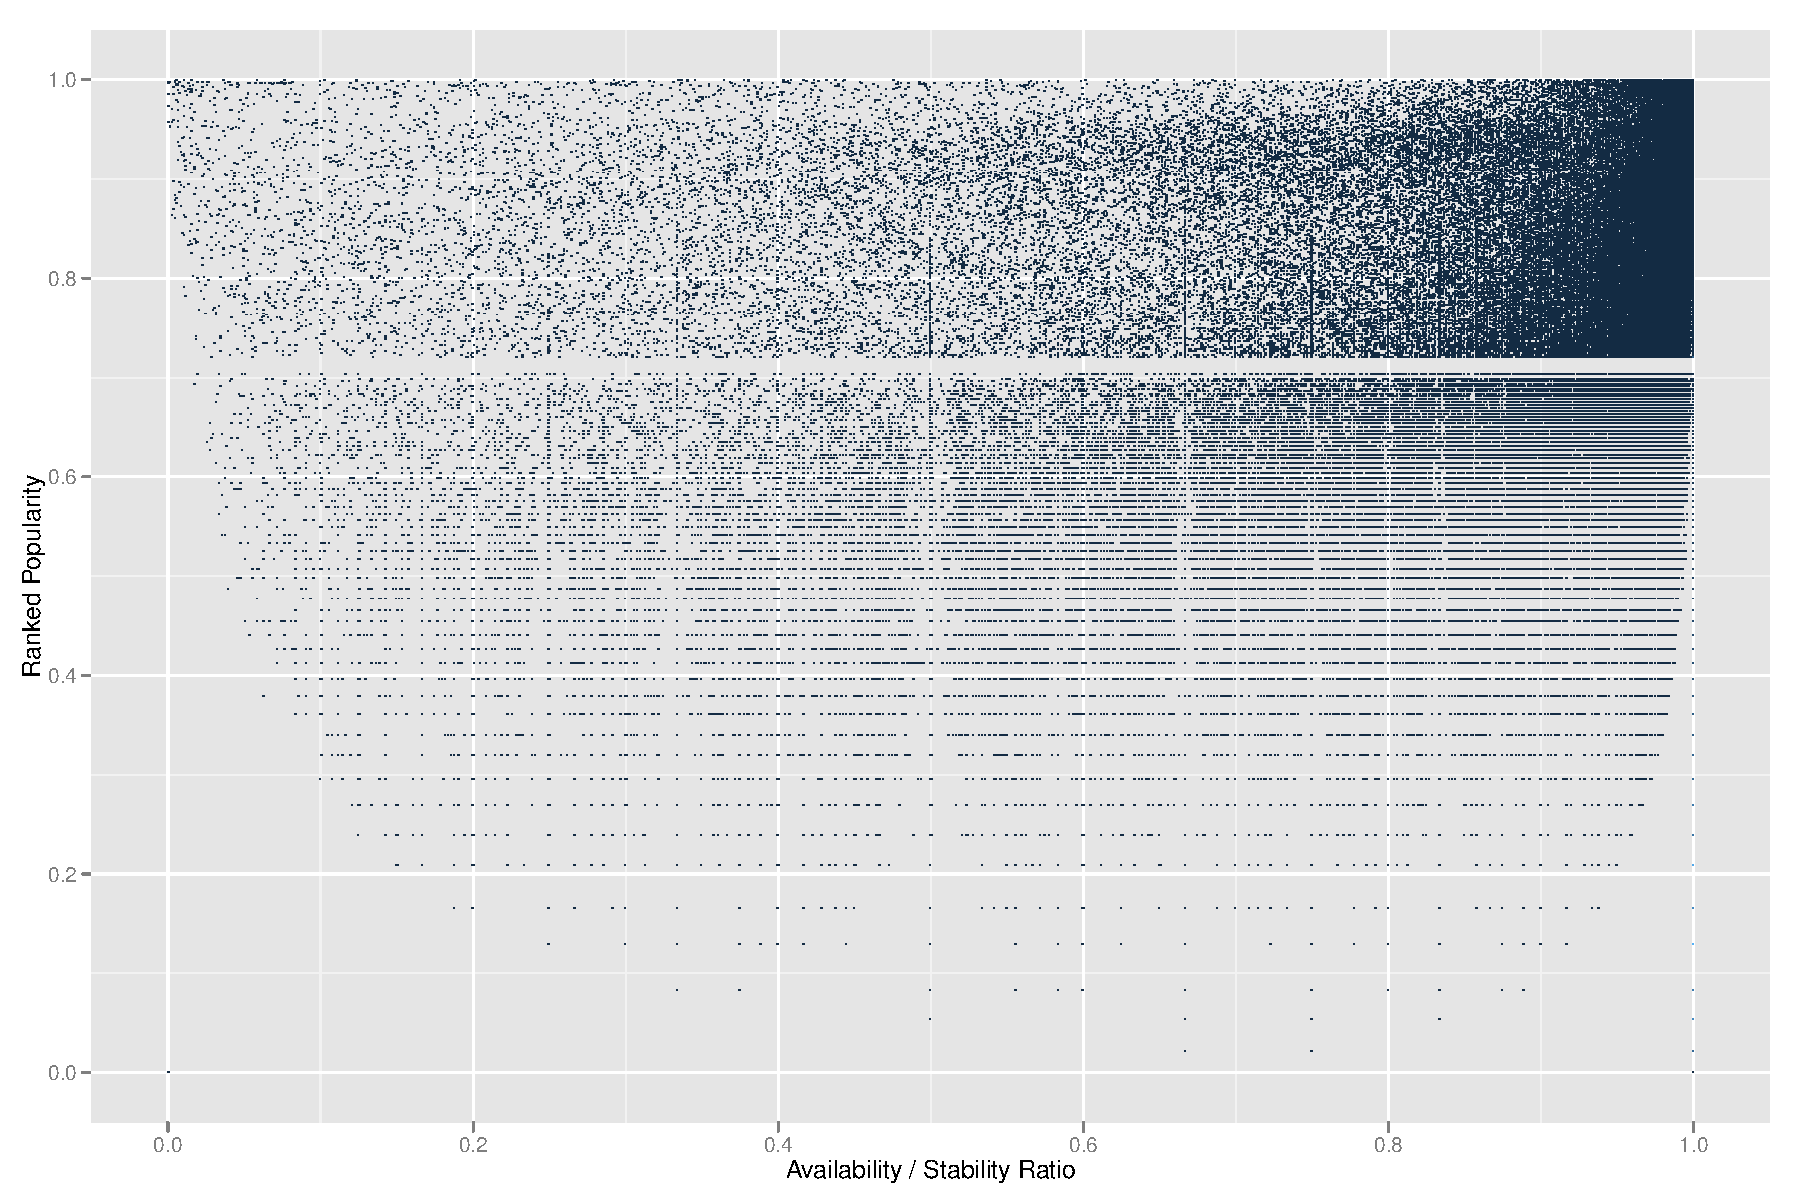
\includegraphics[width=\linewidth]{images/popularity_stability_map.pdf}
	\caption{Sockets by their ranked popularity and their stability} 
	\label{fig:rankedPopularity} 
\end{figure}

\begin{landscape}
	\begin{figure}
	[p] \centering 
	\includegraphics[width=\linewidth]{images/top20_ratio_box.pdf}
	\caption{box-and-whisker plot of the availability / stability of the top 20 traffic port server sockets} 
	\label{fig:top20_ratio_box} 
\end{figure}
\end{landscape}

\begin{landscape}
\begin{figure}
	[p] \centering 
	\includegraphics[width=\linewidth]{images/top20_visibility_box.pdf}
	\caption{box-and-whisker plot of visibility in days of the top 20 traffic port server sockets}
	\label{fig:top20_visibledays_box}
\end{figure}
\end{landscape}

\begin{table}
	[ht] \centering 
	\begin{tabular}
		{|c|r|r|r|r|r|r|} \hline \textbf{Position} & \textbf{Port} & \textbf{Protocol} & \textbf{Flows} &\textbf{ Flows in \%} & \textbf{Sockets} & \textbf{Sockets in \%}\\
		\hline \hline 1 & 53 & 17 &793851107 & 47.272216 & 314253 & 18.68397\\
		\hline 2 & 80 & 6 &623910956 & 37.152626 & 546735 & 32.50623\\
		\hline 3 & 443 & 6 & 74333936 & 4.426434 & 59800 & 3.555420\\
		\hline 4 & 22 & 6 & 10580812 & 0.630066 & 40363 & 2.399790\\
		\hline 5 & 2703 & 6 & 10139578 & 0.603791 & 22 & 0.001308\\
		\hline 6 & 25 & 6 & 6943533 & 0.413473 & 18560 & 1.103488\\
		\hline 7 & 123 & 17 & 4988781 & 0.297072 & 286 & 0.017004\\
		\hline 8 & 993 & 6 & 3844043 & 0.228905 & 1398 & 0.083118\\
		\hline 9 & 555 & 6 & 3290709 & 0.195955 & 9 & 0.000535\\
		\hline 10 & 995 & 6 & 2411245 & 0.143585 & 654 & 0.038884\\
		\hline 11 & 110 & 6 & 1816240 & 0.108153 & 1211 & 0.072000\\
		\hline 12 & 3789 & 6 & 1796224 & 0.106961 & 10 & 0.000595\\
		\hline 13 & 53 & 6 & 1726716 & 0.102822 & 1102 & 0.065520\\
		\hline 14 & 2128 & 6 & 1677027 & 0.099864 & 390 & 0.023188\\
		\hline 15 & 3478 & 17 & 1607132 & 0.095701 & 176 & 0.010464\\
		\hline 16 & 8080 & 6 & 1362615 & 0.081141 & 2056 & 0.122240\\
		\hline 17 & 3128 & 6 & 1298424 & 0.077319 & 191 & 0.011356\\
		\hline 18 & 5354 & 6 & 1221109 & 0.072715 & 3 & 0.000178\\
		\hline 19 & 8001 & 6 & 1014631 & 0.060419 & 58 & 0.003448\\
		\hline 20 & 21 & 6 & 1010771 & 0.060189 & 1419 & 0.084367\\
		\hline 21 & high & 6 & 37679906 & 2.243762 & 599314 & 35.63233\\
		\hline 22 & high & 17 & 89558306 & 5.333015 & 89820 & 5.340265\\
		\hline 23 & low & 6 & 2505504 & 0.149198 & 3807 & 0.226346\\
		\hline 24 & low & 17 & 749276 & 0.044618 & 302 & 0.017955\\
		\hline 
	\end{tabular}
	\caption{Top 20 port / protocol aggregated sockets by number flows}
	\label{tab:top20_ports}
\end{table}\todo{do something with me..}
